%!TEX TS-program = xelatex
%!TEX root = ../../maxwell2018thesis.tex

\chapter[A Background of Stopping in IIR]{A Background of Stopping in\\Interactive Information Retrieval}\label{chap:stopping_background}

In the previous chapter, we provided a high level overview of~\gls{acr:ir}. In particular, we provided a brief history of the area, the basic families of retrieval models, and various measures that have traditionally been used to evaluate the effectiveness of a retrieval system. Towards the end of the chapter, we began to shift from the \emph{system-sided} research that has dominated~\gls{acr:ir} research (and quite understandably so), towards the more \emph{user-centred} research with which the work in this thesis considers. In particular, as alluded to in Chapter~\ref{chap:intro}, and indeed in the title of this thesis, we now turn our attention to the concept of \emph{stopping behaviour} in the context of~\gls{acr:iir}.

\begin{figure}[h]
    \centering
    \vspace{4mm}
    \resizebox{1\hsize}{!}{
    
\includegraphics{figures/ch3-stopsign.pdf}}
    \label{fig:stopsign}
    \vspace{-5mm}
\end{figure}

With many of the models and measures employed in~\gls{acr:ir} and~\gls{acr:iir} research today largely agnostic of a searcher's stopping behaviour, we in this chapter provide an overview of a variety of different \emph{stopping heuristics} that have been defined in the literature over a number of decades, provide a discussion on a number of different user studies that have examined searcher stopping behaviours, discuss basic theoretical frameworks that provide a potential insight and explanation into why people stop, and then discuss a variety of different user models that have been developed that better attempt to model a searcher's interactions, and thus allow for a better representation of their stopping behaviour.

\section{Why Stopping?}
As previously mentioned, knowing when to stop is a fundamental aspect of human thinking and behaviour. Humans and other animals when interacting with the world will employ some form of \emph{stopping criterion} to decide when they should stop~\citep{nickles1995judgment}. As an example, a shopper who is looking to purchase a new smartphone will stop shopping around once he or she has obtained sufficient information on what new smartphone to purchase. Once their case notes for a patient have been compiled, a medical doctor will then be in a position to diagnose the patient's ailment.

The decision of when to stop is not exclusively due to factors external to the decision maker, but rather from a series of \emph{internal, cognitive factors} of their thinking process~\citep{nickles1995judgment}. An individual who is hungry will stop eating once he or she is no longer hungry, rather than stopping when all of the food presented to him or her has been consumed. Empirical research has over the years demonstrated that individuals, regardless of the task presented to them, will frequently stop prematurely. Indeed, this na\"{i}ve behaviour demonstrates that individuals may be willing to go with what \emph{``sounds right''} to them -- often minimising the cognitive effort that is required at the expense of greater accuracy~\citep{perkins1983difficulties}. However, this lower level of potential accuracy does lead searchers to making a greater number of errors in their decision making~\citep{baron1988heuristics}, with individuals overlooking important elements, and potentially miss out useful information~\citep{fischhoff1977cost_benefit, fischhoff1978fault, shafir1992thinking}, with the individual then failing to consider alternatives~\citep{farquhar1993decision_structuring}.

Based upon prior research into the phenomenon of stopping behaviour, it is clear that this is driven primarily from internal factors. As such, we then consider: \emph{what aspects of the decision maker's thinking processes prompt him or her to stop assessing the information provided?} Knowing when to stop requires that the individual in question makes a \emph{judgement} regarding the sufficiency of the information obtained, and whether or not additional information is required to be obtained~\citep{browne2004stopping_rules}. This judgement is normally characterised by both the completeness and correctness of the information obtained thus far~\citep{smith1991belief}. These claims can be mirrored by qualitative studies on examining stopping behaviour, where researchers have found that searchers stop examining a ranked list of results simply because what they have found previously is \emph{``good enough''}~\citep{wu2014information_scent}, echoing the reasoning that individuals will be happy to stop when what they have found \emph{``sounds right''}~\citep{perkins1983difficulties}.

\section{Stopping Heuristics}\label{sec:stopping_background:heuristics}
Considering the above, researchers have over a number of decades devised a number of different high level \emph{stopping rules} -- hereafter referred to as \emph{stopping heuristics} -- as a means of encoding a searcher's aforementioned sense of what is \emph{``good enough''} -- or, indeed, what can be considered to be \emph{not good enough,} too.

Stopping heuristics have been investigated in \emph{decision making} research. A number of normative stopping heuristics have been identified. As examples of such heuristics,~\cite{busemeyer1988deferred_decision_making} considered the expected loss from terminating information acquisition.~\cite{kogut1990sunk_costs} examined the expected value of additional information. Other examples of normative stopping heuristics are demonstrated by~\cite{pitz1969information_seeking} and~\cite{busemeyer1988deferred_decision_making}. However, as outlined by~\cite{browne2004stopping_rules}, these heuristics usually fail to describe the actual cognitive behaviours of the decision makers. Such heuristics often assume that the decision maker must \emph{think ahead} to the final decision of when to stop, enabling them to assess the value of additional information~\citep{busemeyer1988deferred_decision_making}. This is however an inherently difficult task for decision makers to undertake, due to the limited working memory capacity of a human -- we are simply unable to hold and evaluate all of the information attained to make a decision considering all possible outcomes~\citep{browne2004stopping_rules}.~\cite{nickles1995judgment} agreed, stating that normative stopping heuristics made implicit assumptions about the mental activities of the decision maker, especially in terms of mental scaling and weighting. No clear cognitive perspective is provided to address the assumptions of the decision maker's thinking.

With these inherent limitations in mind, seminal work in this area was undertaken by~\cite{nickles1995judgment} who provided a broad classification for different explicitly defined stopping heuristics in the literature that consider a searcher's cognitive processes: \emph{judgement based heuristics} and \emph{reasoning based heuristics.}~\cite{nickles1995judgment} also proposed a number of stopping heuristics that are discussed in subsequent sections, with discussion expanded to included additional heuristics defined by other researchers.

\begin{figure}[t!]
    \centering
    \resizebox{1\hsize}{!}{
    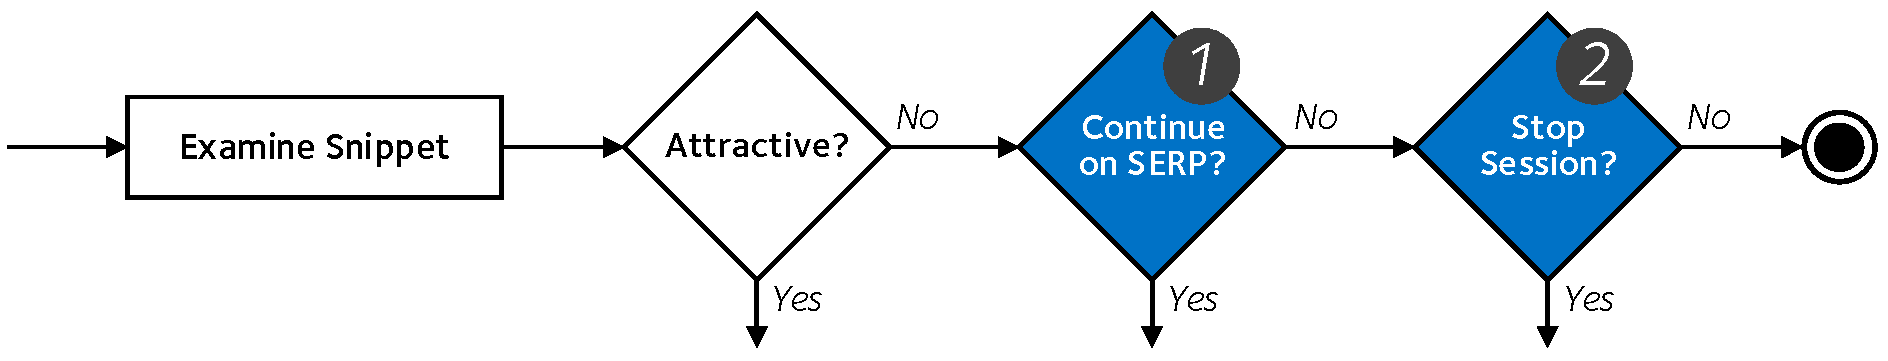
\includegraphics{figures/ch3-two_points.pdf}}
    \caption[Two main stopping decision points of the search process]{An excerpt from a wider user search model, demonstrating two key, established stopping decision points commonly discussed in the literature. These are highlighted in the illustration as {\color{dmax_lightblue}blue} diamonds. The two points consider \blueboxbold{1} \emph{snippet level stopping} (often called \emph{query level stopping}), and \blueboxbold{2} \emph{session level stopping}.}
    \label{fig:model_two_points}
\end{figure}

\noindent\blueboxbold{Considering Stopping Decision Points} It is important to note that in the context of search, stopping heuristics have often been discussed at two key \emph{stopping decision points} in the literature. To demonstrate this, Figure~\ref{fig:model_two_points} illustrates an excerpt from a basic user model that highlights these two key stopping decision points. In the figure, decision point \blueboxbold{1} considers \emph{snippet level stopping} -- often referred to as \emph{query level stopping} in the literature.\footnote{In this thesis, we use the terminology \emph{snippet level stopping} to avoid potential confusion between this well defined stopping decision point, and a further one that we introduce in Chapter~\ref{chap:proposal}.} This stopping decision point addresses the issue of how deep a searcher should examine a ranked list of results presented to him or her on a given SERP. In addition to this, the second stopping decision point, \blueboxbold{2}, as demonstrated in Figure~\ref{fig:model_two_points}, considers wider \emph{session level stopping}. This stopping decision point permits a searcher to determine whether they have met their overall search goal, have run out of time, or have simply become exasperated with the lack of promising results. While these two key stopping decision points are discussed in more detail in Section~\ref{sec:proposal:stopping_points}, it should be noted that the heuristics defined in this section can be applied to snippet level stopping, session level stopping, or both.

\subsection{Judgement Based Heuristics}
A judgement based stopping heuristic is defined as when a decision maker is assumed to set and consistently maintain a mental threshold along some form of key dimension (e.g. determining the seemingly relevant from non-relevant), and to keep a running total of measure relative to the dimension in question~\citep{gettys1979hypothesis, nickles1995judgment}. When the measure is met or exceeded this set threshold, the searcher then stops and proceeds to the next step, or abandons the search altogether. A number of different judgement based heuristics have been defined in the literature, the most prominent of which we discuss here.

\subsubsection{Satisfaction and Frustration}
Two of the earliest stopping heuristics defined in the literature are by~\cite{cooper1973retrieval_effectiveness_ii} which consider a searcher's tolerance to relevant and non-relevant material. The heuristics were originally defined as a means for estimating the utility a searcher can attain when interacting with a search system. While the means of which~\cite{cooper1973retrieval_effectiveness_ii} estimated the utility of search are not of key relevance to this thesis, the work on stopping heuristics are. The \emph{satisfaction point} and \emph{frustration point} stopping heuristics are considered to be judgement based heuristics, as they rely solely on the searcher's notion of what constitutes a relevant document -- and both consider counts of the number of (non-)relevant documents observed.

\noindent\blueboxbold{Satisfaction Point}
Given the name, it is not surprising that the \emph{satisfaction point} rule considers the point at which a searcher has found enough perceived relevant material to consider his or her search a success. It can be easily imagined that such a rule would apply directly to both snippet level stopping (i.e. \emph{find $x$ relevant documents on this SERP}) and session level stopping (i.e. \emph{find $x$ relevant documents}). This heuristic is also called the \emph{satiation heuristic} (see below).

\noindent\blueboxbold{Frustration Point}
In a converse fashion to the satisfaction point heuristic, the \emph{frustration point} heuristic considers a searcher's overall \emph{tolerance to non relevance}, by stopping after being sufficiently frustrated by the results presented to the searcher. This heuristic is also called the \emph{disgust heuristic} in the literature (see below).

The two relatively straightforward heuristics defined above makes a searcher's interactions with a ranked list of results, or SERPs, \emph{inherently adaptive.} Given a set of results, his or her behaviour will change with respect to the perceived quality of the ranked list of results. As a reminder, this would not necessarily mean considering the system's effectiveness measures, but rather user-focused measures such as interactive precision and recall (refer to Section~\ref{sec:ir_background:user:evaluation:interactive_pr}).

\noindent\blueboxbold{Combining Satisfaction and Frustration}
Perhaps due to the relative simplicity of these heuristics, identical approaches have also been defined elsewhere in the literature.~\cite{kraft1979stopping_rules} later defined three further stopping heuristics, two of which are the \emph{satiation} and the somewhat loaded \emph{disgust} heuristics. In essence, the rules defined by~\cite{kraft1979stopping_rules} are the same satisfaction and disgust heuristics as previously defined by~\cite{cooper1973retrieval_effectiveness_ii}. Within the satiation rule, a searcher will stop after been \emph{satiated} by finding a number of documents considered to be relevant, while the disgust rule considers a searcher's disgust at finding a number of non-relevant documents.

\cite{kraft1979stopping_rules} also proposed a third heuristic that \emph{combines} both the satisfaction/satiation and frustration/disgust rules together into a single heuristic. Here, a searcher following such an approach would be inclined to stop examining content if they were either satisfied with what had been found, or frustrated by having to trawl through a number of material judged to be non-relevant. The stopping point would be whatever of the two conditions are met first. Indeed,~\cite{kraft1979stopping_rules} demonstrated that the expected search length of a searcher could be approximated using each of the two stopping heuristics by considering the size of the retrieval set, the number of relevant documents a searcher wished to obtain, and the number of non-relevant documents a searcher would be willing to tolerate. The number of documents required to consider a search as successful is dependent upon whether the search task is high precision (where one would stop comparatively early), or high recall (where one would stop comparatively later), as hypothesised by~\cite{bates1984thirty_items}.

\subsubsection{Magnitude Threshold}
The magnitude threshold heuristic, as outlined by~\citep{nickles1995judgment}, considers an individual's belief that the information accrued during the search process provides sufficient \emph{evidence} to prompt him or her to stop searching for information. The point at which the searcher would decide to stop is determined by some predetermined, internal threshold that must be reached, which acts as the stopping criterion~\citep{wald1948sequential_analysis, nickles1995judgment}.~\cite{gettys1979hypothesis} hypothesise that the searcher \emph{`mentally tabulates'} the cumulative impact of the evidence that he or she has uncovered, and when the internal tabulation crosses the specified threshold, he or she stops.

Determining what exactly this threshold should be before commencing a task has attracted research from several perspectives. Indeed, this decision can be left open to interpretation by the individuals who choose to operationalise such a heuristic. However, research has shown that under different tasks, varying the criteria by which an individual bases their initial threshold value varies. For example,~\cite{busemeyer1982choice_behaviour} demonstrated this for decision making under uncertainty.~\cite{saad1996stopping} demonstrated the usefulness of this heuristic under common choice tasks.

\begin{wrapfigure}{r}{0.45\textwidth}
    \begin{center}
    \vspace*{-10mm}
    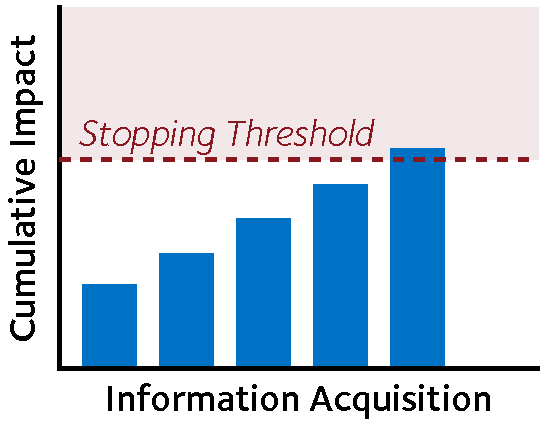
\includegraphics[width=1\textwidth]{figures/ch3-threshold.pdf}
    \end{center}
    \vspace*{-4mm}
    \caption[The magnitude threshold stopping heuristic]{The magnitude threshold stopping heuristic. Once a searcher accrues a predetermined level of impact, he or she stops. Figure adapted from~\cite{browne2004stopping_rules}.}
    \label{fig:threshold}
\end{wrapfigure}

An abstract representation of the stopping heuristic is provided in Figure~\ref{fig:threshold}. From the figure, we can see that a searcher accrues information through each document that is examined. This is combined together to form a \emph{cumulative impact} for the information. For each document examined, the current cumulative impact value is compared against a predetermined threshold value -- if the cumulative impact appears to be above the threshold, the searcher then assumes that enough supporting evidence has been collected, and subsequently stops.

\subsubsection{Difference Threshold}
Again outlined by~\citep{nickles1995judgment}, the \emph{difference threshold heuristic} concerns whether a new document is teaching a searcher anything new about their given information need, or the marginal value of the latest document. Here, the searcher is assumed to keep an internal record of the cumulative impact of information that has been consumed along some key dimension. The searcher is also assumed to use this internal record of what has been assessed to compare a new document with previously examined content. When the absolute difference between the two assessments falls below some internal difference threshold, the searcher would then stop as nothing new is being learnt.

\begin{figure}[t!]
    \centering
    \resizebox{1\hsize}{!}{
    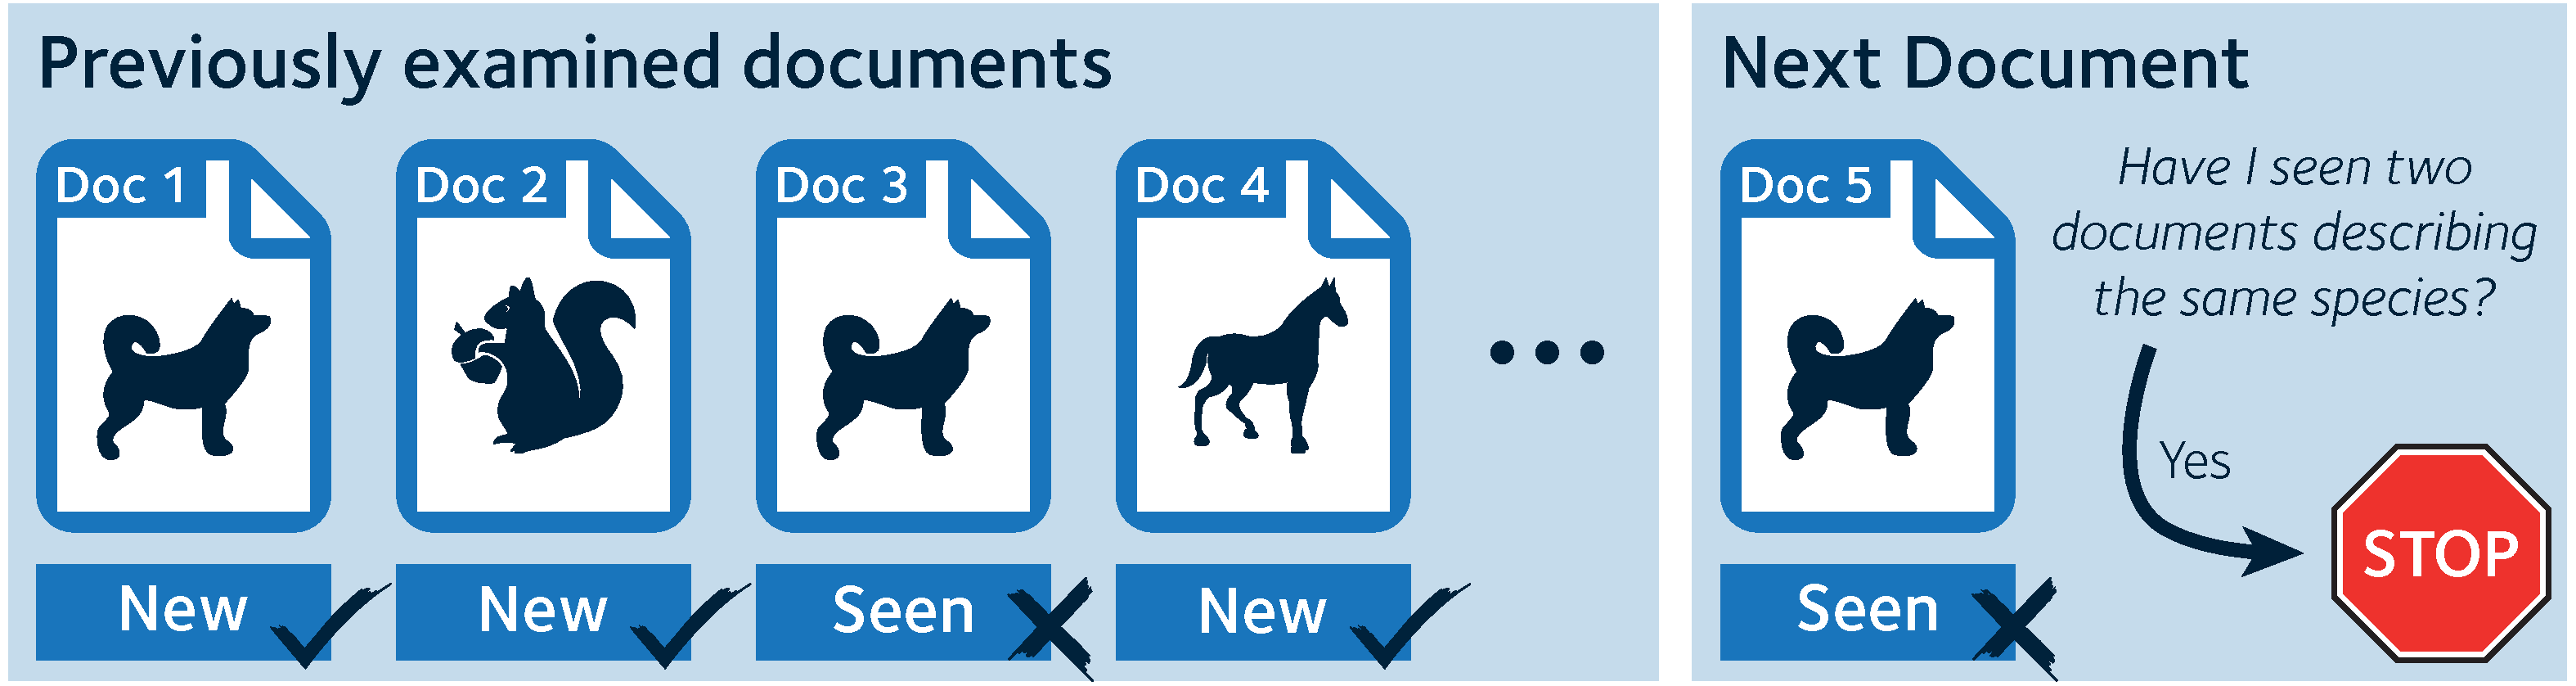
\includegraphics{figures/ch3-difference.pdf}}
    \caption[Difference threshold heuristic]{A simplified, visual example of the difference threshold heuristic. Given the information need of finding different species of animal, a searcher issues a query, and examined a number of documents. The third document offers information on dogs, which has been already observed in \blueboxbold{Doc 1}. Using the stopping criterion that once the same species has been observed twice, \blueboxbold{Doc 5} satisfies it – and thus, the searcher stops.}
    \label{fig:difference_heuristic}
\end{figure}

As a crude example of this heuristic, a searcher is provided with an information need to find as many different species of animal as possible. Once a query has been issued, the searcher begins to examine documents on the SERP. This is illustrated in Figure~\ref{fig:difference_heuristic}, where the first document considers dogs. A simple criterion is employed whereby the searcher stops after encountering the same animal twice, illustrating that nothing new is being learnt from the list of results presented. Once this is met, the searcher abandons the SERP, and can then perform a query reformulation to discover different species of animal.

\subsubsection{Single Criterion}
The \emph{single criterion heuristic} was later defined by~\cite{browne2005stopping_rules}. As the name suggests, this heuristic considers a searcher examining information for a \emph{single criterion} related to their information need, typically assumed to be the most important one. The searcher then stops examining content once he or she has deduced that enough information about said criterion has been accumulated for them to be satisfied. The concept of a stopping threshold can be borrowed from the magnitude threshold heuristic. This considers that a searcher will stop once they have accumulated enough impactful information.

\cite{browne2005stopping_rules} go on to provide an example search task where the single criterion threshold would be directly applicable. When purchasing a mortgage for a new house, a searcher will explore various mortgage lender's websites in order to find the best deal. Given a mortgage deal, the most obvious criterion that an individual would look for would be interest rates -- the lower, the more attractive the deal. Of course, other factors may influence the decision, but this example ultimately demonstrates a potential application of the heuristic.

\subsection{Reasoning Based Heuristics}
The second category of stopping heuristics as defined by~\citep{nickles1995judgment} are \emph{reasoning based}. While searching and accruing information about a particular topic, a searcher is essentially developing a form of mental representation of the various elements of the topic as he or she learns~\citep{yates1990decision_making}. As argued by~\citep{nickles1995judgment}, these elements can include arguments constructed during informal reasoning, previously constructed arguments, or information evoked from the searcher's long term memory. As such,~\citep{nickles1995judgment} devised a category of stopping heuristics that are dominated by the searcher's reasoning processes.

\subsubsection{Representational Stability}
\begin{wrapfigure}[8]{r}{0.45\textwidth}
    \begin{center}
    \vspace*{-10mm}
    
\includegraphics[width=1\textwidth]{figures/ch3-representational.pdf}
    \end{center}
    \vspace*{-4mm}
    \caption[Representational stability stopping heuristic]{A crude illustration of the representational stability stopping heuristic. The searcher's model of the given information need begins to stabilise at \emph{t-1}, meaning that a searcher would stop at \emph{t}.}
    \label{fig:representational_heuristic}
\end{wrapfigure}

This heuristic concerns the notion that as a search acquires new information via the search process, his or her mental model of the underlying information need shifts and develops -- but only up to a certain point. From this point where their mental model stabilises, the searcher is said to have accrued enough information to satisfy their information need.

The notion of representational stability is based upon the stopping heuristic outlined by~\cite{nickles1995judgment}, the phenomenon of which is initially discussed by~\cite{yates1982toward}.~\cite{nickles1995judgment} argues that while a searcher examines content, he or she generates arguments that serve to develop and elaborate his or her conception of the decision(s) that they are tasked to make. As the searcher continues to reason, certain arguments may be relegated to long term memory due to the limited size of the searcher's working memory. As the information seeking process continues, constructs arguments from this information and accommodates his or her mental model of the information need, the searcher may at some point return to the same subset of arguments. As mentioned previously, it is at this point that can be interpreted as a form of stability regarding the information need. This is crudely demonstrated in Figure~\ref{fig:representational_heuristic}, where given a vague information need, a searcher will trawl a series of documents in order to develop their mental model of the given problem.

\subsubsection{Propositional Stability}
Similar to the representational stability heuristic,~\cite{nickles1995judgment} also defined the \emph{propositional stability} heuristic again focuses on the concept of a stabilising mental model of the given information need. Here, a searcher when examining content will form a series of arguments from the information he or she is observing. These arguments can lead to \emph{tentative conclusions}, from which at some point stability is achieved, and the conclusion does not change. This heuristic therefore suggests that the stabilised nature of the decision maker's conclusion from the information observed prompts him or her to stop.

\subsubsection{Mental List}
This final reasoning based stopping heuristic concerns the notion of a searcher constructing a mental list of items or aspects of a particular item that they are attempting to search for. Each of the different items within the mental list must be checked off to a satisfactory level before the searcher then decides to stop examining content. This mental list can typically be constructed from a searcher's long term memory -- meaning that they will likely have \emph{a priori} knowledge of the particular information need. So-called belief structures such as \emph{schema}~\citep{bartlett1933remembering} or \emph{scripts}~\citep{schank1977scripts} may assist the searcher in organising the construction of the mental list that will form the set of criteria that determines when they stop.

Figure~\ref{fig:mental_list} provides a graphical illustration of the mental list heuristic. When looking for a new car, a searcher will construct a mental list of different aspects of a car which are essentially the minimum requirements (e.g. a minimum engine displacement of 1.8 litres). Searching is then conducted, with the searcher narrowing down the potential choices available to them to those that satisfy their mental list.

\begin{figure}[t!]
    \centering
    \resizebox{1\hsize}{!}{
    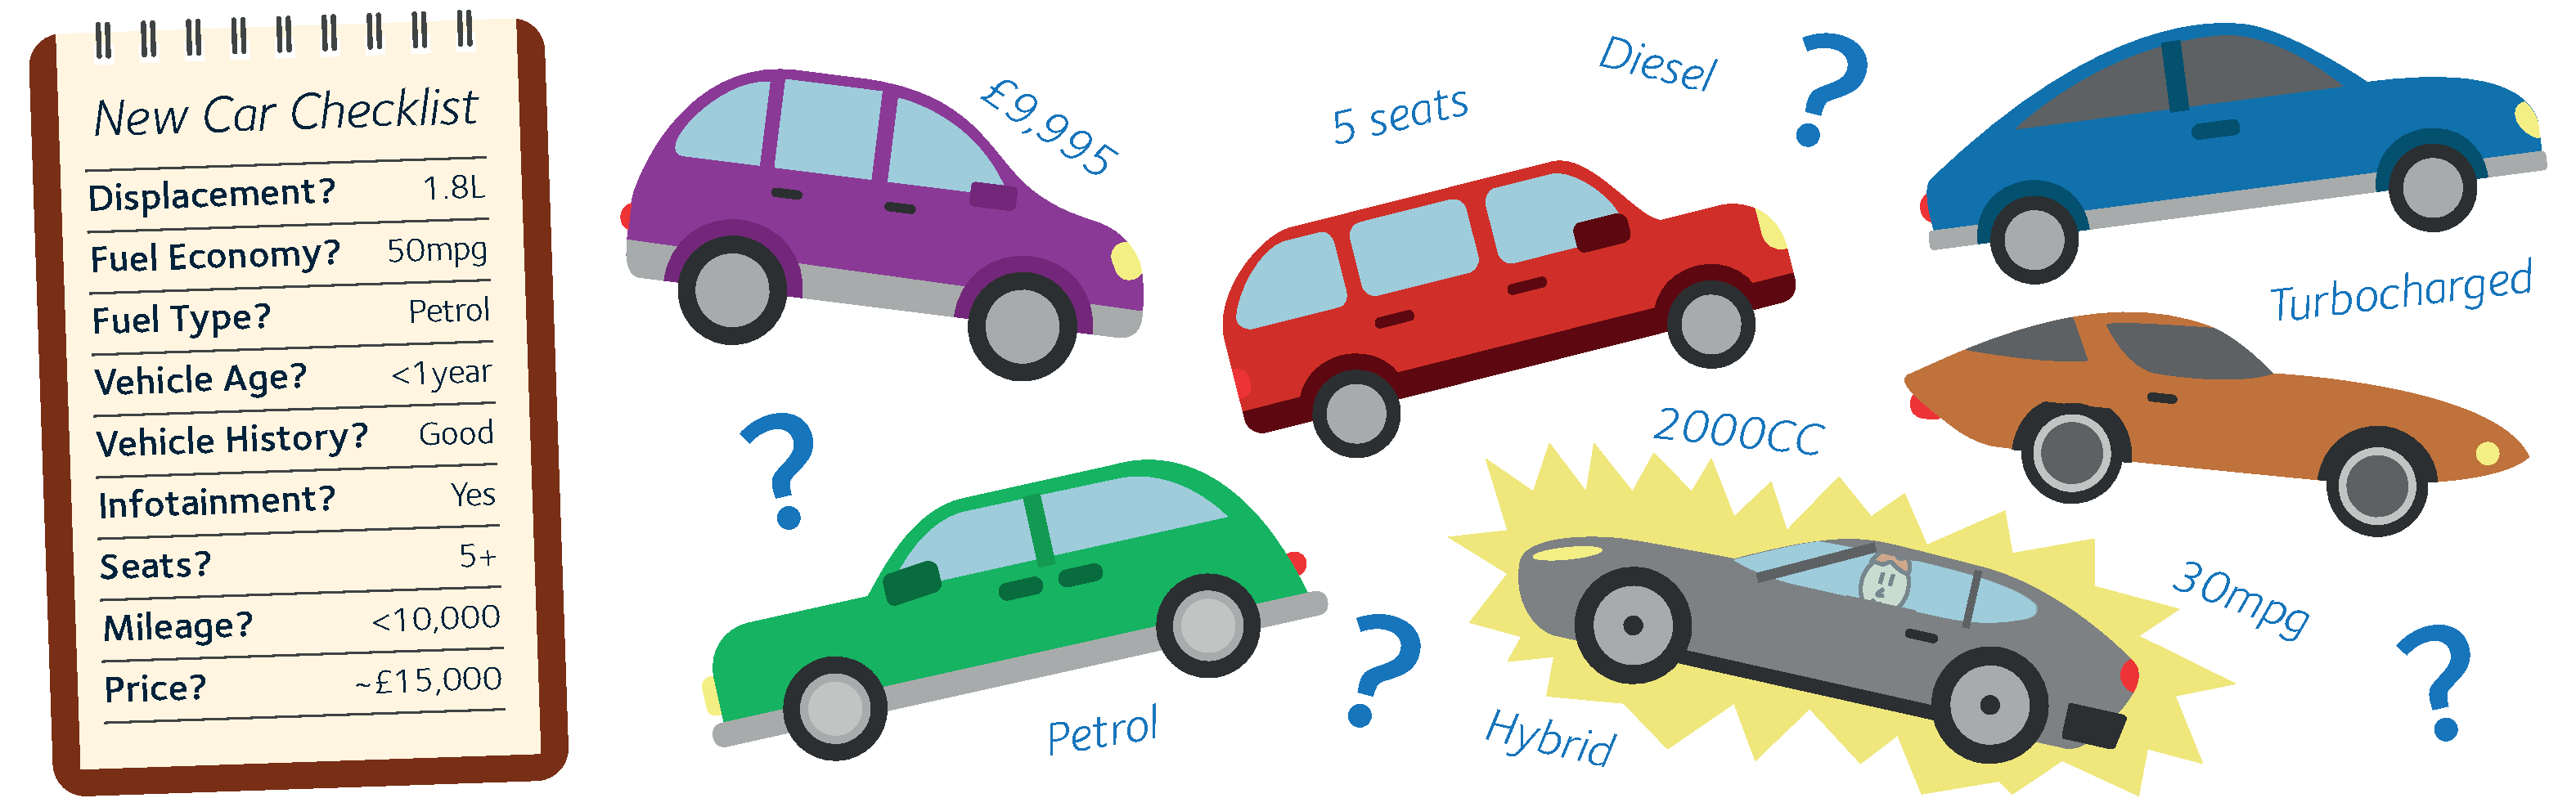
\includegraphics{figures/ch3-mental_list.pdf}}
    \caption[The mental list stopping heuristic]{Given a well defined information need,~\cite{nickles1995judgment} defined the mental list heuristic – where a number of different criteria must be satisfied before stopping. In the illustration above, car shopping is used as an example. Here, certain criteria for a new car (as shown on the notepad) must be met before a searcher is satisfied with what they have found.}
    \label{fig:mental_list}
\end{figure}

\subsection{Summary of Heuristics}
In this section, a number of different stopping heuristics have been discussed from a number of seminal papers in the literature. While a much larger of number of normative stopping heuristics have been defined in prior works, these have been omitted from the review as they do not adequately describe the cognitive behaviours of a searcher, often assuming a searcher has to \emph{think ahead} to make a decision to stop or continue~\citep{browne2004stopping_rules}. In contrast, the heuristics that are enumerated above do not make this assumption, making more realistic assumptions about the searcher's cognitive abilities.

Of course, the different stopping heuristics discussed above are likely to behave differently under different search contexts. As an example, the mental list heuristic might be impossible to use given a searcher with a very limited knowledge of a topic. He or she simply would not know enough information to ascertain key aspects of the topic, and construct a set of criteria that must be met~\citep{browne2005stopping_rules} --~\cite{gigerenzer1999betting} also discuss this reasoning for the single criterion heuristic. As such, it is hypothesised that the aforementioned stopping heuristics would be likely to work better with a searcher who is more knowledgeable. Indeed,~\cite{browne2005stopping_rules} hypothesises that magnitude threshold and mental list heuristics would be best applied to searchers with a greater degree of understanding of the topic.

\cite{browne2005stopping_rules} also discuss the so-called \emph{``structuredness''} of a given search task. If the task has well defined inputs and outputs -- or the goals and operations are clear and easily understood~\citep{simon1996sciences} -- then it it hypothesised that searchers will employ more precise stopping heuristics for deducing when to stop. For example, the mental list and single criterion stopping heuristics might offer greater degrees of precision than for example the frustration and satisfaction heuristics, although the frustration and satisfaction heuristics may perform well for any given search task. Altogether however, the heuristics discussed in this section would all be applicable for information search~\citep{browne2005stopping_rules}.

With the heuristics now enumerated, we later in this thesis discuss how we take the heuristics, and consider how to \emph{operationalise} them, such that they can be subsequently implemented and compared against each other in an empirical way. Refer to Section~\ref{sec:proposal:strategies} for the complete set of \emph{stopping strategies} that we employ.

\section{User Studies}

studies from CIKM 2015 paper.

ryen white's expert stuff -- does he report stopping stuff?

depth first vs breadth first??

conceptual models (e.g. following on from TREC, we end up with...thomas, baskaya...), then move on to theoretical models

like we mentioned in Ch2, in the different measures, we have different stopping rules encoded within them.
e.g. Carterette's 2011 model.


\section{User Models of Search}
In addition to the key stopping heuristics and user studies associated with examining a searcher's stopping behaviour, \emph{models of search} are also of paramount importance to the work detailed in this thesis. Models of search were briefly touched upon in Section~\ref{sec:ir_background:user:models}, with particular reference to the TREC-style approach of user modelling. There, we queried whether this model of search \emph{was particularly realistic.}

This is a question that has been asked my many~\gls{acr:ir} researchers, and as a result, much work has been undertaken in this area in an attempt to develop our understanding of the processes that are undertaken by searchers during an interactive search session. In this section, we discuss a broad variety of models that are of particular relevance to the work discussed later in this thesis. We discuss two broad strands of user models: those that are \emph{conceptual} in nature, and those that are based on more \emph{theoretical} foundations.

% so there are also developments in how people search, examining different activities.
% we look at wider models of search, encapsulating different components of the search process.
%
% From more conceptual, to theoretical.
%
% What about the attention model in ``Beyond ten blue links: enabling user click modeling in federated web search''?
%
% here are some implicit models (e.g. Azzo 2011)

\subsection{Conceptual Models}\label{sec:stopping_background:models:conceptual}
Put simply, a conceptual model is a representation of some system, \emph{comprised} of a series of concepts that can be used to help us learn, understand or \emph{simulate} what the model represents. In the context of~\gls{acr:iir}, models comprise of the different activities that a searcher undertakes during the search process. Examples include issuing a query, and examining document(s) for relevance. In this section, we discuss several key models that have been developed by researchers over a number of decades. Some of these models are explicitly or implicitly defined within the literature, as discussed in Section~\ref{sec:ir_background:user:simulation}.

\subsubsection{The TREC User Model}\label{sec:stopping_background:models:conceptual:trec}
Thus far, we have discussed the notion that within \blueboxbold{TREC-style studies}, we argue that there is the notion of an underlying user model that is exploited to produce the list of results from a given~\gls{acr:ir} system that can then be subsequently evaluated. This model is typically used in a batch environment, where many queries are issued in turn.

\begin{figure}[t!]
    \centering
    \resizebox{1\hsize}{!}{
    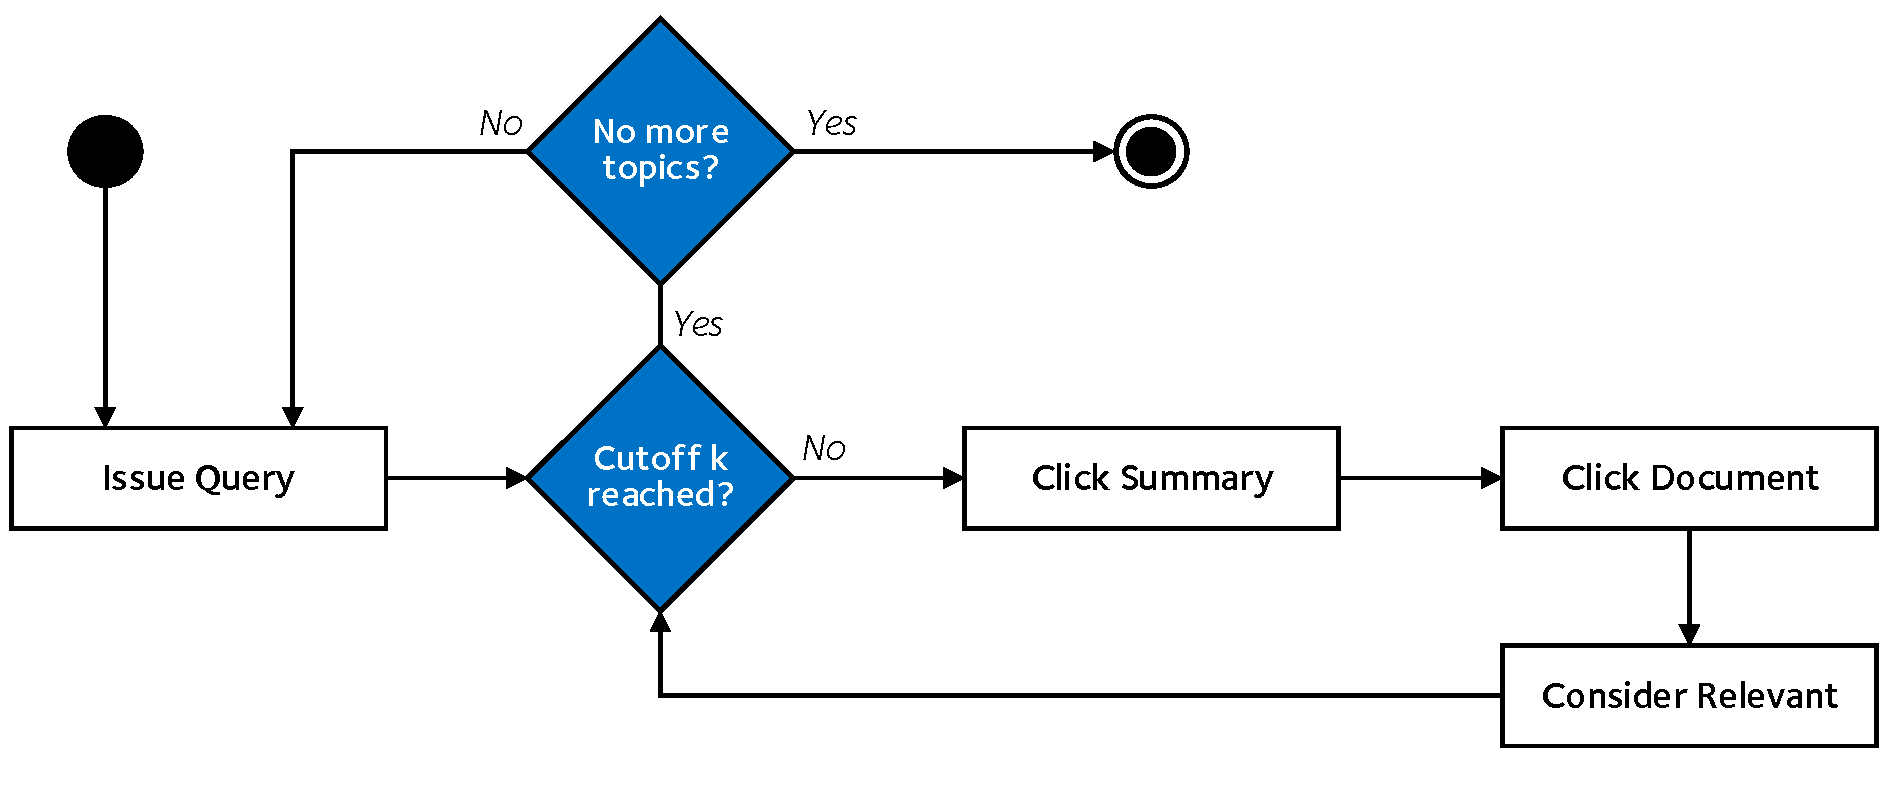
\includegraphics{figures/ch2-trec.pdf}}
    \caption[The TREC-style user model]{A basic flowchart of the user model typically encoded within TREC-style experimentation. \emph{'Users'} subscribing to this model will issue a query – typically the title of a topic – and then proceed to examine results to some fixed depth, $k$.}
    \label{fig:trec_model}
\end{figure}

A basic flowchart of the user model is presented in Figure~\ref{fig:trec_model}. With a given information need, a searcher (or system) will then translate that information need into some form of query -- from most TREC tasks, the title of a topic is used (as discussed in Section~\ref{sec:ir_background:basics:cranfield}). The query is then issued to the underlying retrieval engine, and a set of results are then returned. From this point on, the process, as alluded to above, is \emph{batch-like} in nature. Every result summary presented is `clicked', with the document subsequently considered relevant, up to some cutoff at $k$. Typically for TREC-style experimentation, this cutoff will be $k=1000$. Once this process has been completed, the next query will be issued to the underlying retrieval engine, until the list of queries have been exhausted. Once this process has been completed, the list of documents considered relevant to the information need (i.e. all $k$ documents) are passed to the evaluation stage of the Cranfield model (refer to Figure~\ref{fig:ir_cranfield}), where the various evaluation measures that are to be used can be calculated.

The question one should ask considering this TREC-style user model is: \emph{is this model particularly realistic?} Arguments can obviously be made for and against such a model, but the general consensus in the~\gls{acr:ir} community is that it is \emph{not} particularly representative of a searcher in real life, regardless of the search task. A number of strong assumptions are made of the behaviour of the searcher, namely that:

\begin{itemize}
    \item{a single query is issued to address a given information need;}
    \item{a searcher subscribing to this model will \emph{always} examine to a fixed depth in the presented results (their \emph{stopping behaviour}); and}
    \item{a searcher will always consider an item presented to him/her as relevant to their information need.}
\end{itemize}

These assumptions have over the years been proven to be largely unrealistic through empirical evidence. For example, searchers will often adapt their stopping behaviour depending upon the quality of the list of results presented.~\cite{borlund2003iir_model} also puts forward the notion that the model does not consider a searcher's \emph{dynamic information needs}. Here, his or her understanding of a particular topic will evolve over time as content is examined and their mental model evolves. The TREC-style model of search considers that the only point at which a searcher `learns' is at the querying stage.

While deficient in terms of considering a searcher's behaviours, the TREC-style model has worked well for the batch-style experimentation that is typically employed at such evaluation forums. It can be argued that the entire process is essentially \emph{simulating} a user, albeit in a limited way.

\subsubsection{Increasing User Model Complexity}
To this end, a number of studies have over the years developed more complex (and arguably more realistic) models of the search process, encapsulating a greater number of concepts within them. In this section, we provide a brief overview of several key advancements in the field, discussing the concepts and advantages that each \emph{evolution} of the searcher model presents.



- recap on the TREC model.
- number of different simulated studies have 




A conceptual model is a representation of a system, made of the composition of concepts which are used to help people know, understand, or simulate a subject the model represents. It is also a set of concepts.

- begin with a reminder of the TREC model, as per Figure~\ref{fig:trec_model} on page~\pageref{fig:trec_model}.

\begin{figure}[t!]
    \centering
    \resizebox{1\hsize}{!}{
    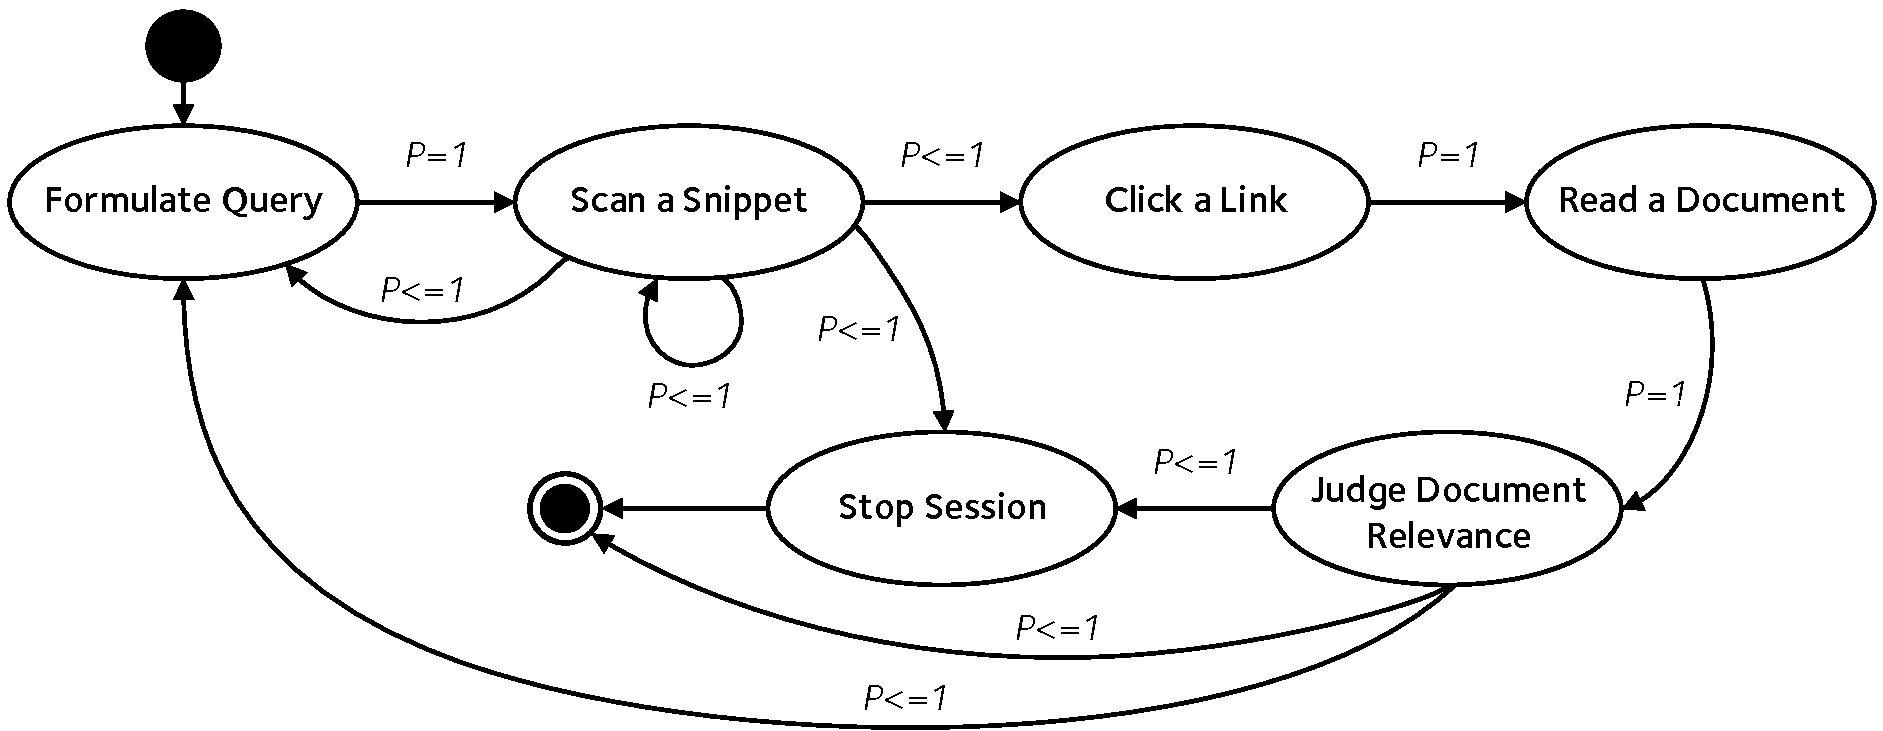
\includegraphics{figures/ch3-baskaya.pdf}}
    \caption[Model of the search process by~\cite{baskaya2013behavioural_factors}]{The user model of search, as outlined by~\citealt{baskaya2013behavioural_factors}. Represented as a Markov Model, the model considers six steps in all. Encoded within two of the steps are decision points that a user following this model must consider in order to continue. Figure adapted (with permission) from the authors of~\citealt{baskaya2013behavioural_factors}.}
    \label{fig:baskaya_model}
\end{figure}

\begin{figure}[t!]
    \centering
    \resizebox{1\hsize}{!}{
    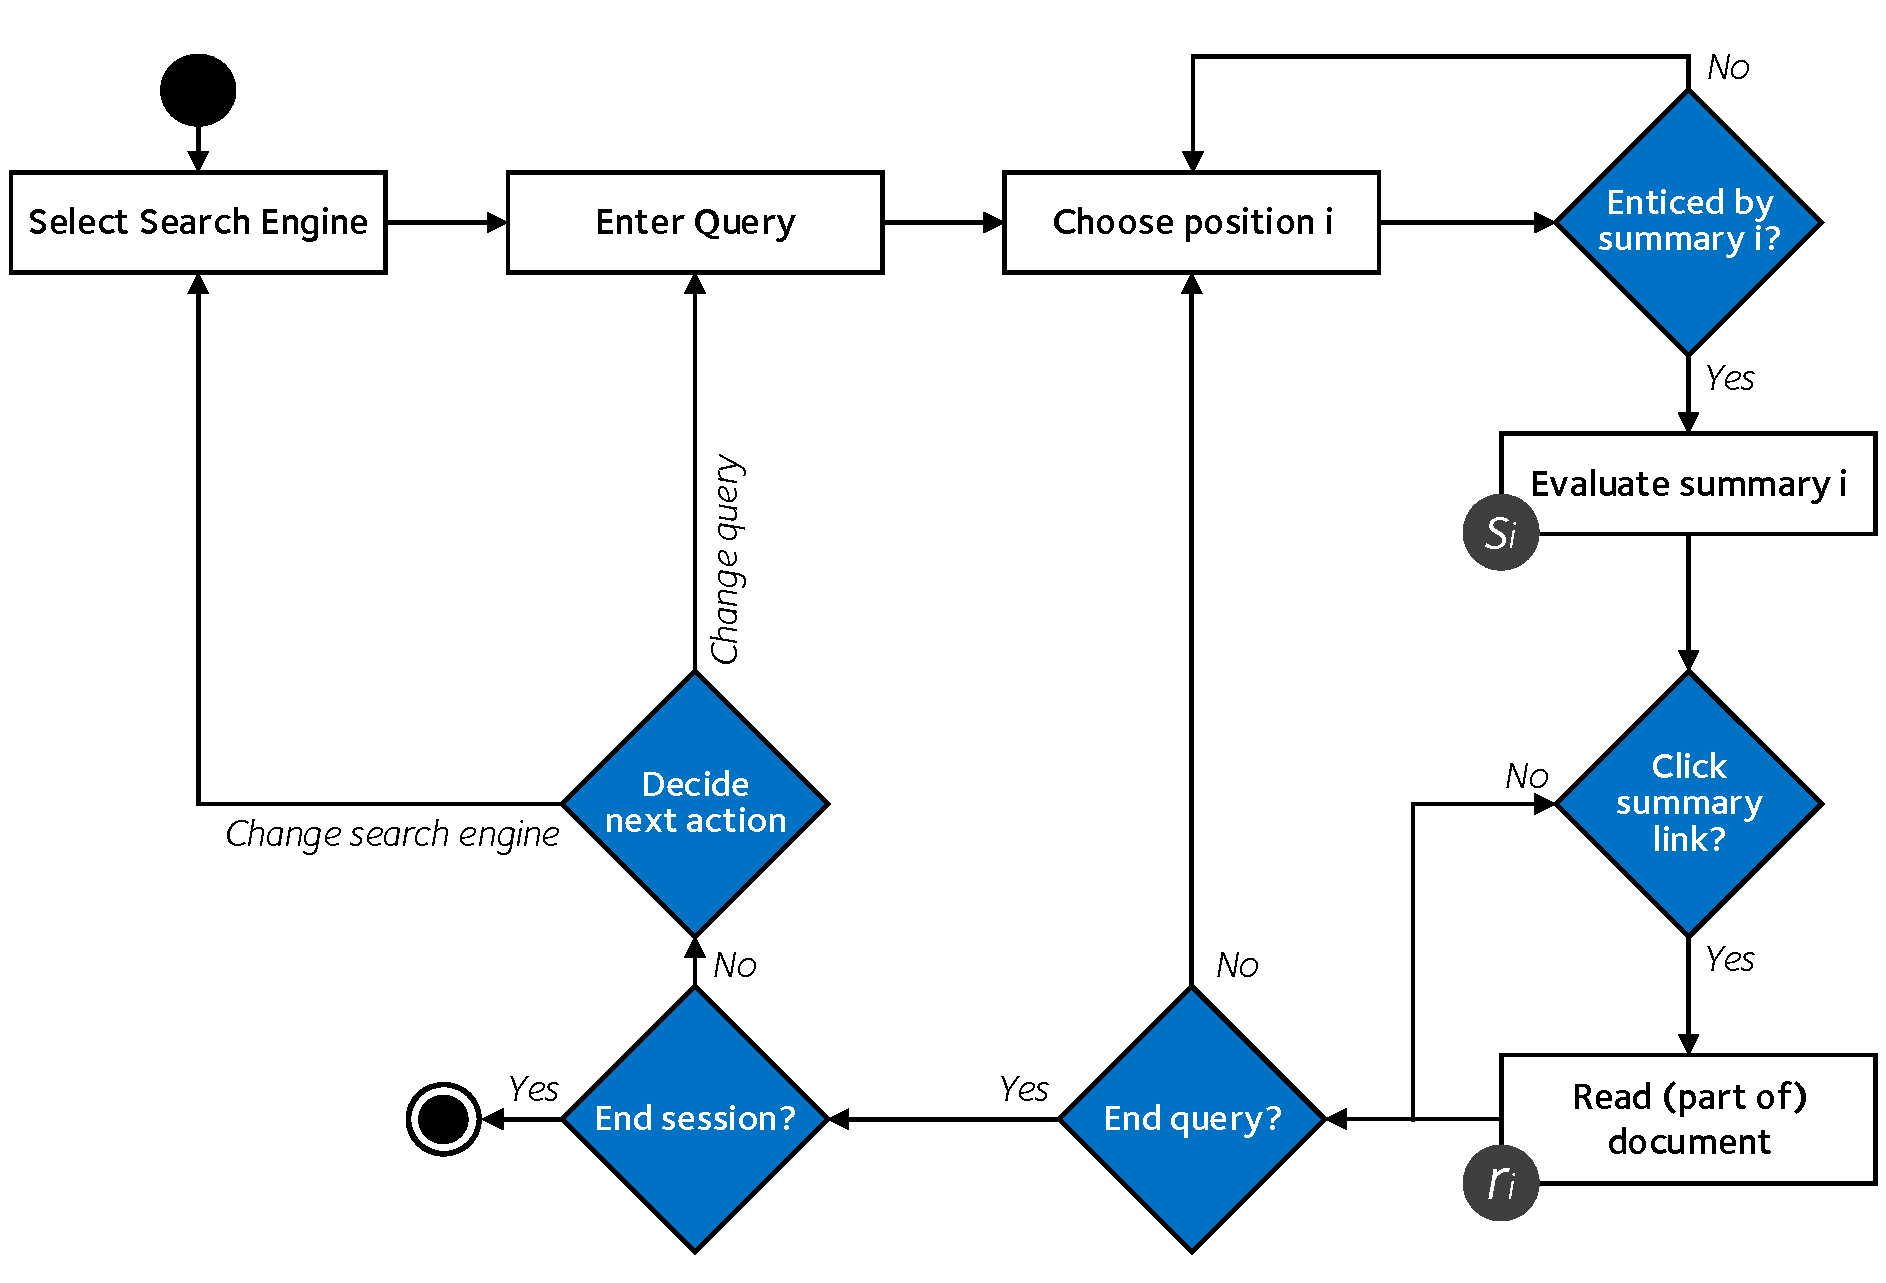
\includegraphics{figures/ch3-thomas.pdf}}
    \caption[Model of the search process by~\cite{thomas2014modelling_behaviour}]{A model of the search process, considering the high-level processes undertaken by a searcher, as outlined by~\cite{thomas2014modelling_behaviour}. Also included are a number of decision points (represented as diamonds) that searchers must consider when following this model. Figure adapted (with permission) from the authors of~\citealt{thomas2014modelling_behaviour}. \textcopyright~Paul Thomas, Peter Bailey, Alistair Moffat and Falk Scholer.}
    \label{fig:thomas_model}
\end{figure}

\subsection{Theoretical Models}

\subsection{Search Economic Theory}

\subsection{Information Foraging Theory}

\subsubsection{Information Patch}

\begin{figure}[t!]
    \centering
    \resizebox{1\hsize}{!}{
    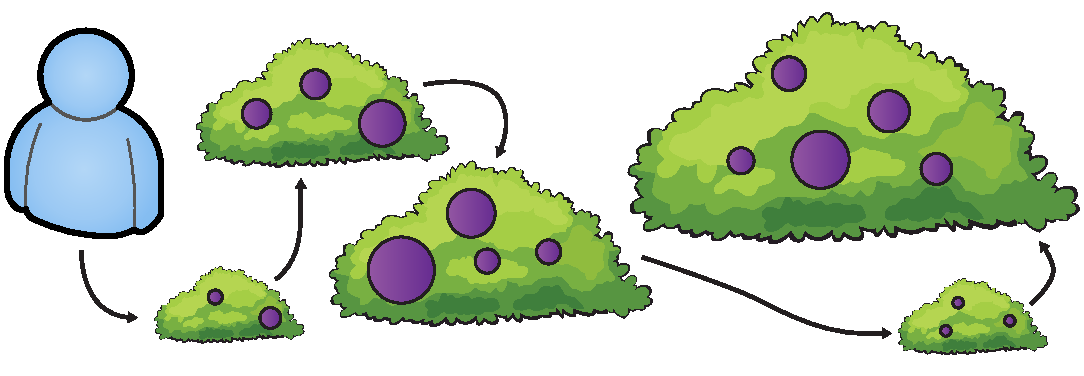
\includegraphics{figures/ch3-berry_picking.pdf}}
    \caption[The Berry Picking Model~\cite{bates1989berry_picking}]{The \emph{Berry Picking Model,} defined by~\cite{bates1989berry_picking}. A forager traverses through numerous bushes to pick the juiciest berries for his or her consumption. The model is high level and conceptual in nature, and thus does not provide any justification for \emph{how} or \emph{why} foragers search for the juiciest berries.}
    \label{fig:berry_picking}
\end{figure}

\subsubsection{Information Scent}

\subsubsection{Considering Stopping Behaviour}

\section{Chapter Summary}
Refer to the following chapter for more information on how we extend these models to make them more realistic.

% - given you an outline of the basics of IR
% - and more system-sided IR
%
% - including a discussion on some of the various measures that are used
% - still very naive in terms of \emph{stopping behaviour}. i.e. assume fixed depths, typically naive about relevance.
%
% - so in this chapter, we begin to consider things from the central point of this thesis - stopping during search.
%
%
%
% - to this end, we in this chapter discuss:
%
% - a variety of different stopping heuristics
% - discuss the basic theories that can be used to explain one's stopping behaviour;
% - and explain the results from different user studies examining a searcher's stopping behaviour
%
% - we then take time to examine
%
% - some of the more complex models of search which are better able to capture stopping.
% 
% \section{Stopping Heuristics}\label{sec:stopping_background:heuristics}
%
% \section{User Studies}
% ryen white's expert stuff -- does he report stopping stuff?
%
% depth first vs breadth first??
%
% conceptual models (e.g. following on from TREC, we end up with...thomas, baskaya...), then move on to theoretical models
%
% like we mentioned in Ch2, in the different measures, we have different stopping rules encoded within them.
% e.g. Carterette's 2011 model.
%
% \section{Models of Search}
%
% \subsection{Conceptual Models}
% The Berry Picking Model
%
% \begin{figure}[t!]
%     \centering
%     \resizebox{1\hsize}{!}{
%     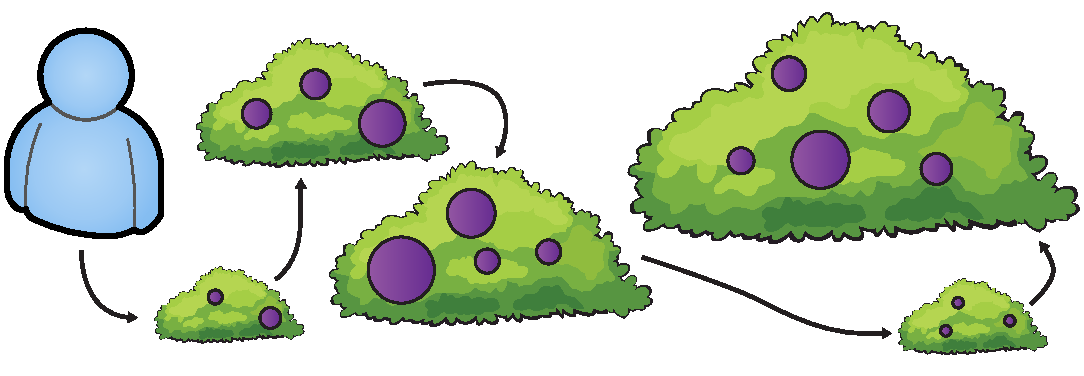
\includegraphics{figures/ch3-berry_picking.pdf}}
%     \caption[The Berry Picking Model~\cite{bates1989berry_picking}]{The Berry Picking Model, defined by~\citealt{bates1989berry_picking}.}
%     \label{fig:berry_picking}
% \end{figure}
%
%
% \subsection{Information Foraging Theory}
%
% \subsection{(Interactive) Probability Ranking Principle}
%
% \subsection{Search Economic Theory}
%
% \subsection{Simple TREC User Model}
%
% \subsection{Paul Thomas Model}
%
% \subsection{Feza Model}
%
% Need to illustrate that there is a development of the user model here.
%
% What about the attention model in ``Beyond ten blue links: enabling user click modeling in federated web search''?
%
% \begin{figure}[t!]
%     \centering
%     \resizebox{1\hsize}{!}{
%     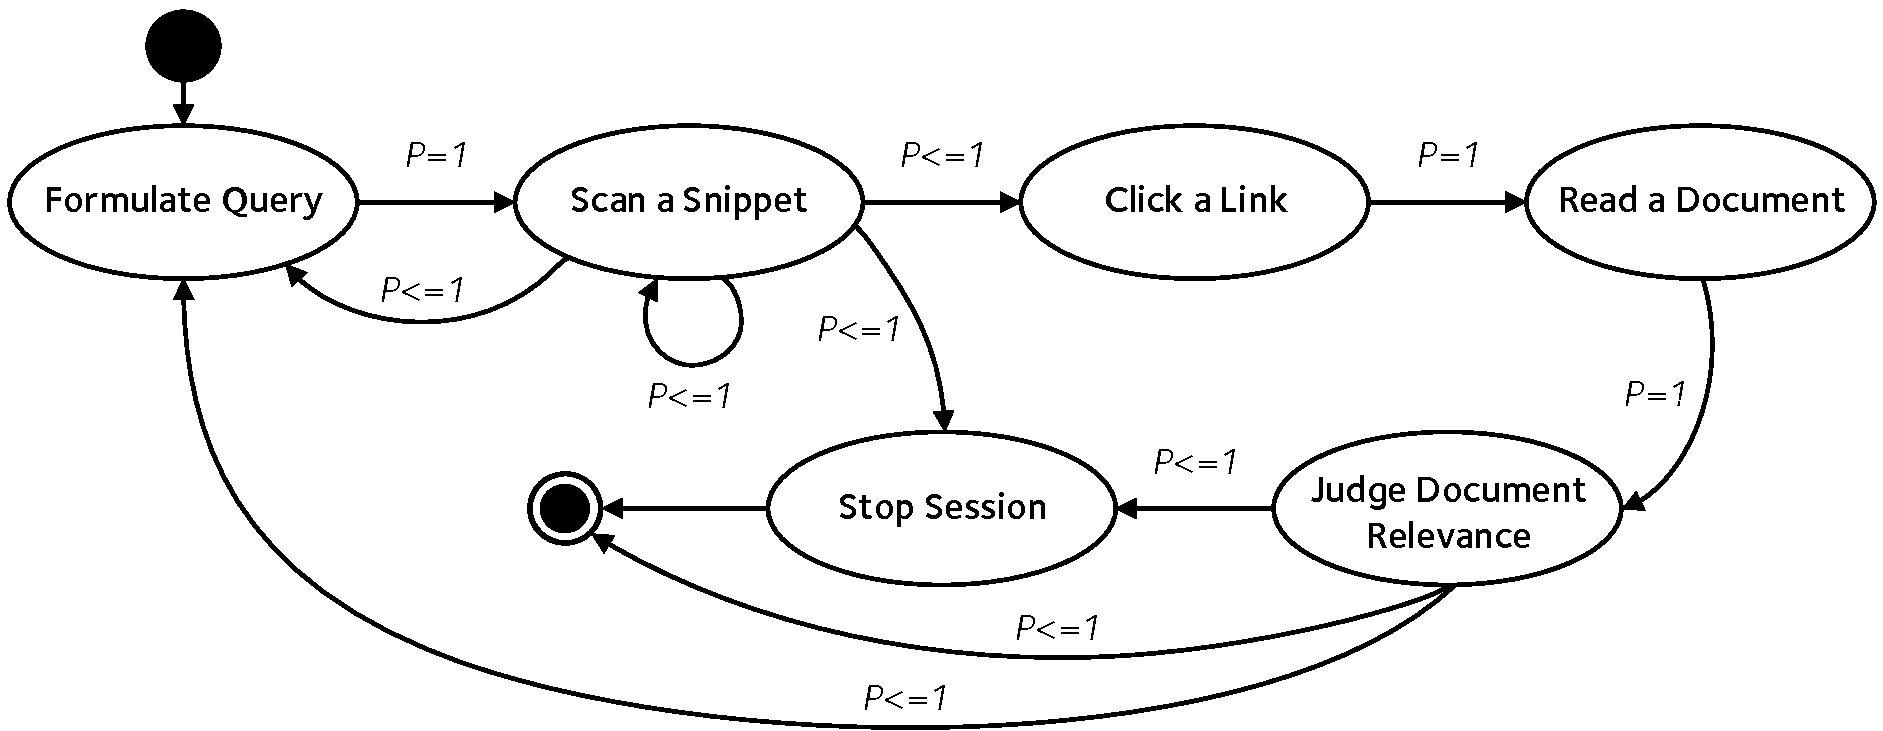
\includegraphics{figures/ch3-baskaya.pdf}}
%     \caption[Model of the search process by~\cite{baskaya2013behavioural_factors}]{The user model of search, as outlined by~\citealt{baskaya2013behavioural_factors}. Represented as a Markov Model, the model considers six steps in all. Encoded within two of the steps are decision points that a user following this model must consider in order to continue. Figure adapted (with permission) from the authors of~\citealt{baskaya2013behavioural_factors}.}
%     \label{fig:baskaya_model}
% \end{figure}
%
% \begin{figure}[t!]
%     \centering
%     \resizebox{1\hsize}{!}{
%     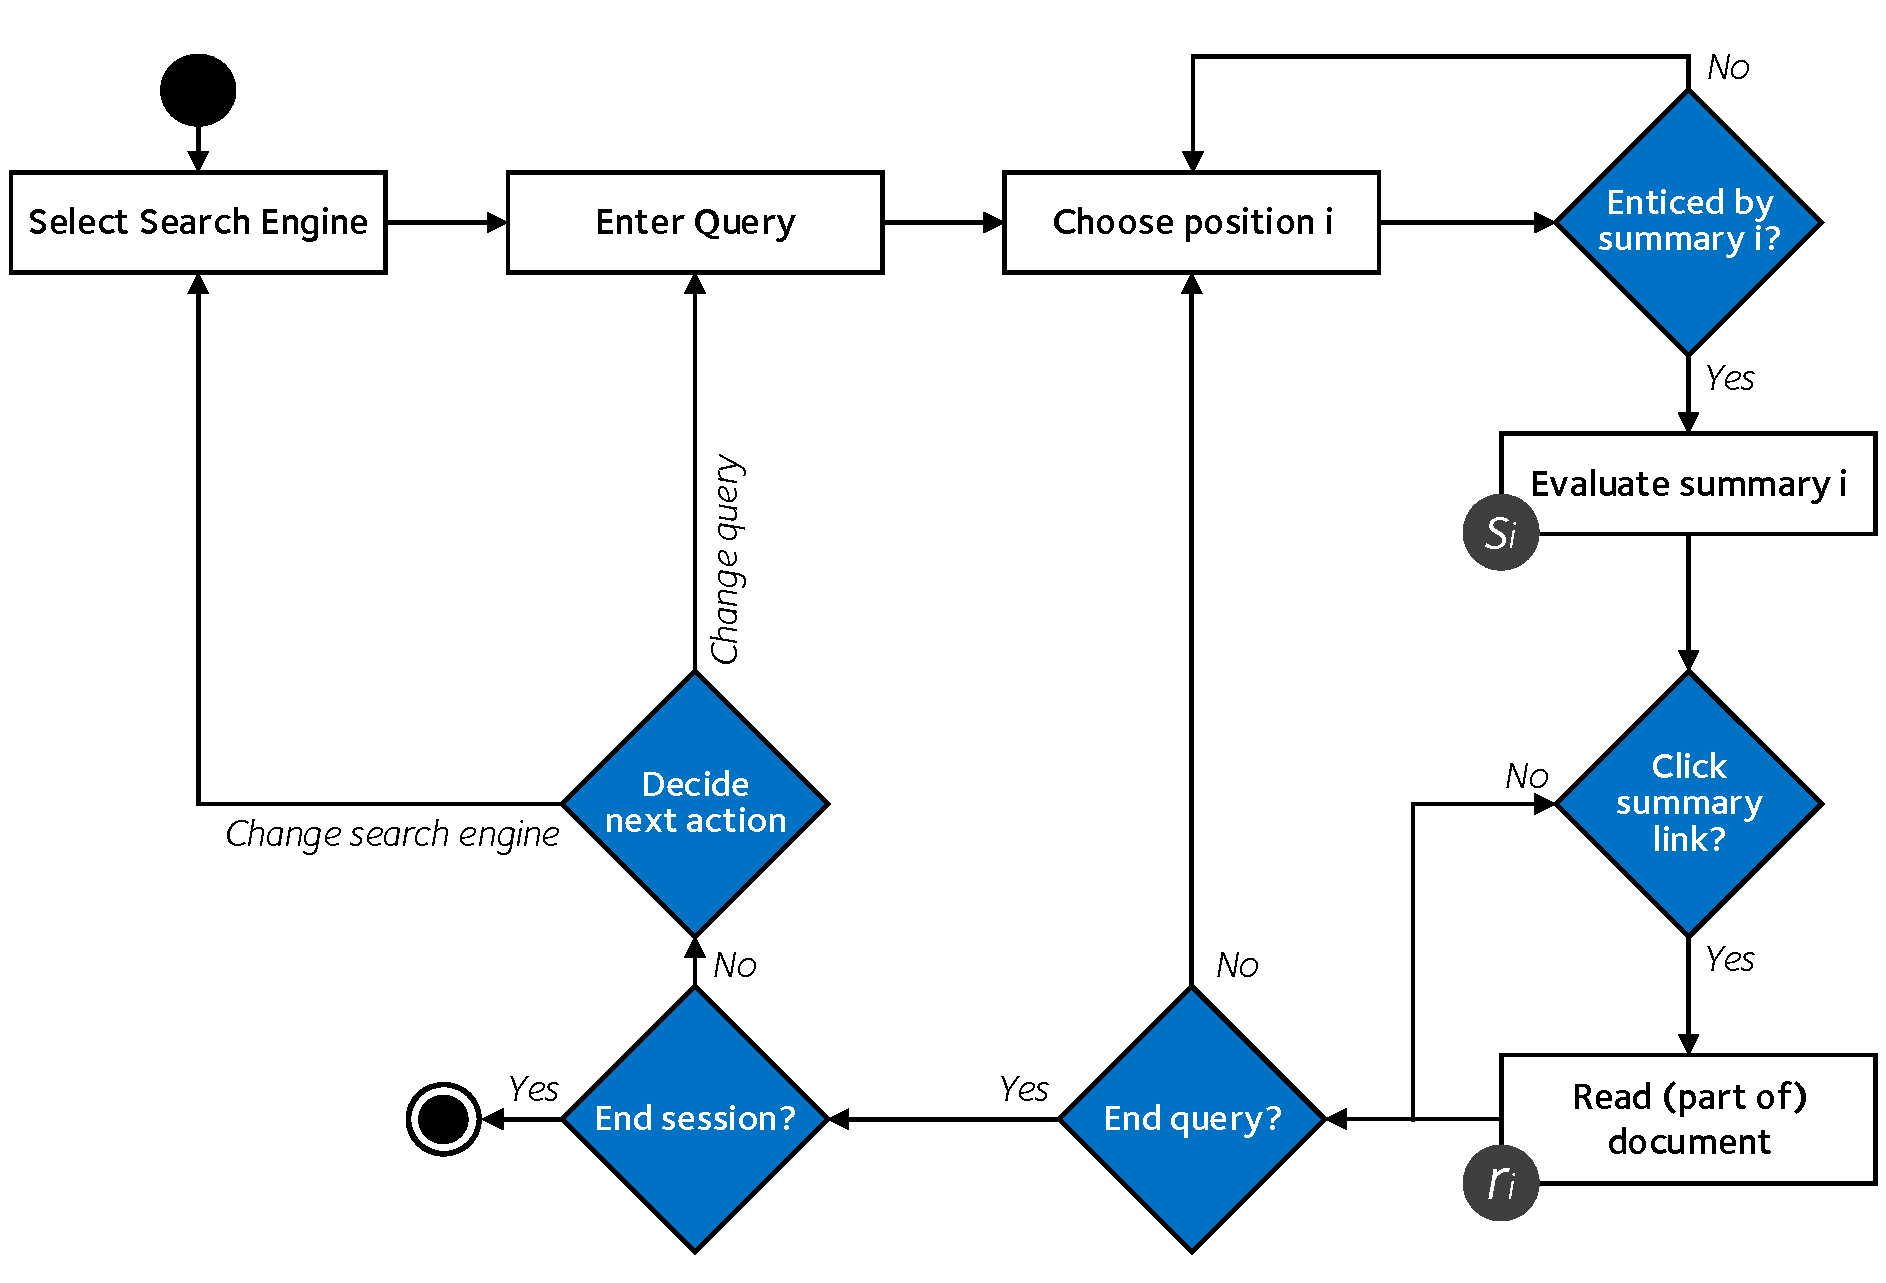
\includegraphics{figures/ch3-thomas.pdf}}
%     \caption[Model of the search process by~\cite{thomas2014modelling_behaviour}]{A model of the search process, considering the high-level processes undertaken by a searcher, as outlined by~\cite{thomas2014modelling_behaviour}. Also included are a number of decision points (represented as diamonds) that searchers must consider when following this model. Figure adapted (with permission) from the authors of~\citealt{thomas2014modelling_behaviour}. \textcopyright~Paul Thomas, Peter Bailey, Alistair Moffat and Falk Scholer.}
%     \label{fig:thomas_model}
% \end{figure}
%
%
% Refer to the following chapter for more information on how we extend these models to make them more realistic.
%
